\documentclass[12pt,a4paper]{article}
\usepackage[utf8]{inputenc}
\usepackage{amsmath}
\usepackage{textcomp}

\usepackage{geometry}
\geometry{a4paper,left=25mm,right=25mm, top=2cm, bottom=2cm} 

\usepackage{verbatim}

 \usepackage{mathptmx}
 \usepackage[scaled=.90]{helvet}
 \usepackage{courier}

\usepackage[utf8]{inputenc}

\usepackage{listings}
\usepackage{color}

\usepackage{graphicx}
 
\definecolor{dkgreen}{rgb}{0,0.6,0}
\definecolor{gray}{rgb}{0.5,0.5,0.5}
\definecolor{mauve}{rgb}{0.58,0,0.82}

\pagestyle{empty}
\lstset{numbers=left,language=C++}
\lstset{showstringspaces=false,
basicstyle=\ttfamily\footnotesize,
breaklines=true,
tabsize=3,
commentstyle=\color{dkgreen},       % comment style
}

%keine einrückungen bei absatz
\parindent 0pt

\begin{document}
\title{Übung 4}
\author{Bernhard Selymes, Reinhard Penn}
\date{November 2012}

\normalsize

%Pfad zu c++ Dateien
\newcommand{\CodePath}{../ImageProcessing/ImageProcessing/}

%Beginn des Dokuments
\section{Organisatorisches}

\subsection{Team}
	\begin {itemize} 
		\item Reinhard Penn, s1110306019 
		\item Bernhard Selymes, s1110306024
	\end {itemize}

\subsection{Aufteilung}
	\begin {itemize} 
		\item Reinhard Penn
			\begin {itemize}
				\item Planung
				\item Klassendiagramm
				\item Implementierung der Klassen SingletonBase, ImageManagement, Circle, EmptyGraphicObjectFactory
				\item Testen aller Klassen
			\end {itemize}
		\item Bernhard Selymes
			\begin {itemize}
				\item Planung
				\item Klassendiagramm
				\item Implementierung der Klassen Image, Rectangle, FilledGraphicObjectFactory, GraphicObject
				\item Dokumentation			
			\end {itemize}
	\end {itemize}


\subsection{Zeitaufwand}
	\begin {itemize}
		\item geschätzte Mh: 20h
		\item tatsächlich: Reinhard (11h), Bernhard  (11h)
	\end {itemize}


\section{Systemspezifikation}

Es soll eine Software für die Erzeugung und Verwaltung von Bildern mit graphischen Objekten erstellt werden. Die Bilder sind in einer Bildverwaltung abgelegt. SVG-Dateien der Bilder können erzeugt werden. Diese können dann in einem Browser angezeigt werden.
\\

\newpage
\section {Systementwurf}

\subsection {Klassendiagramm}

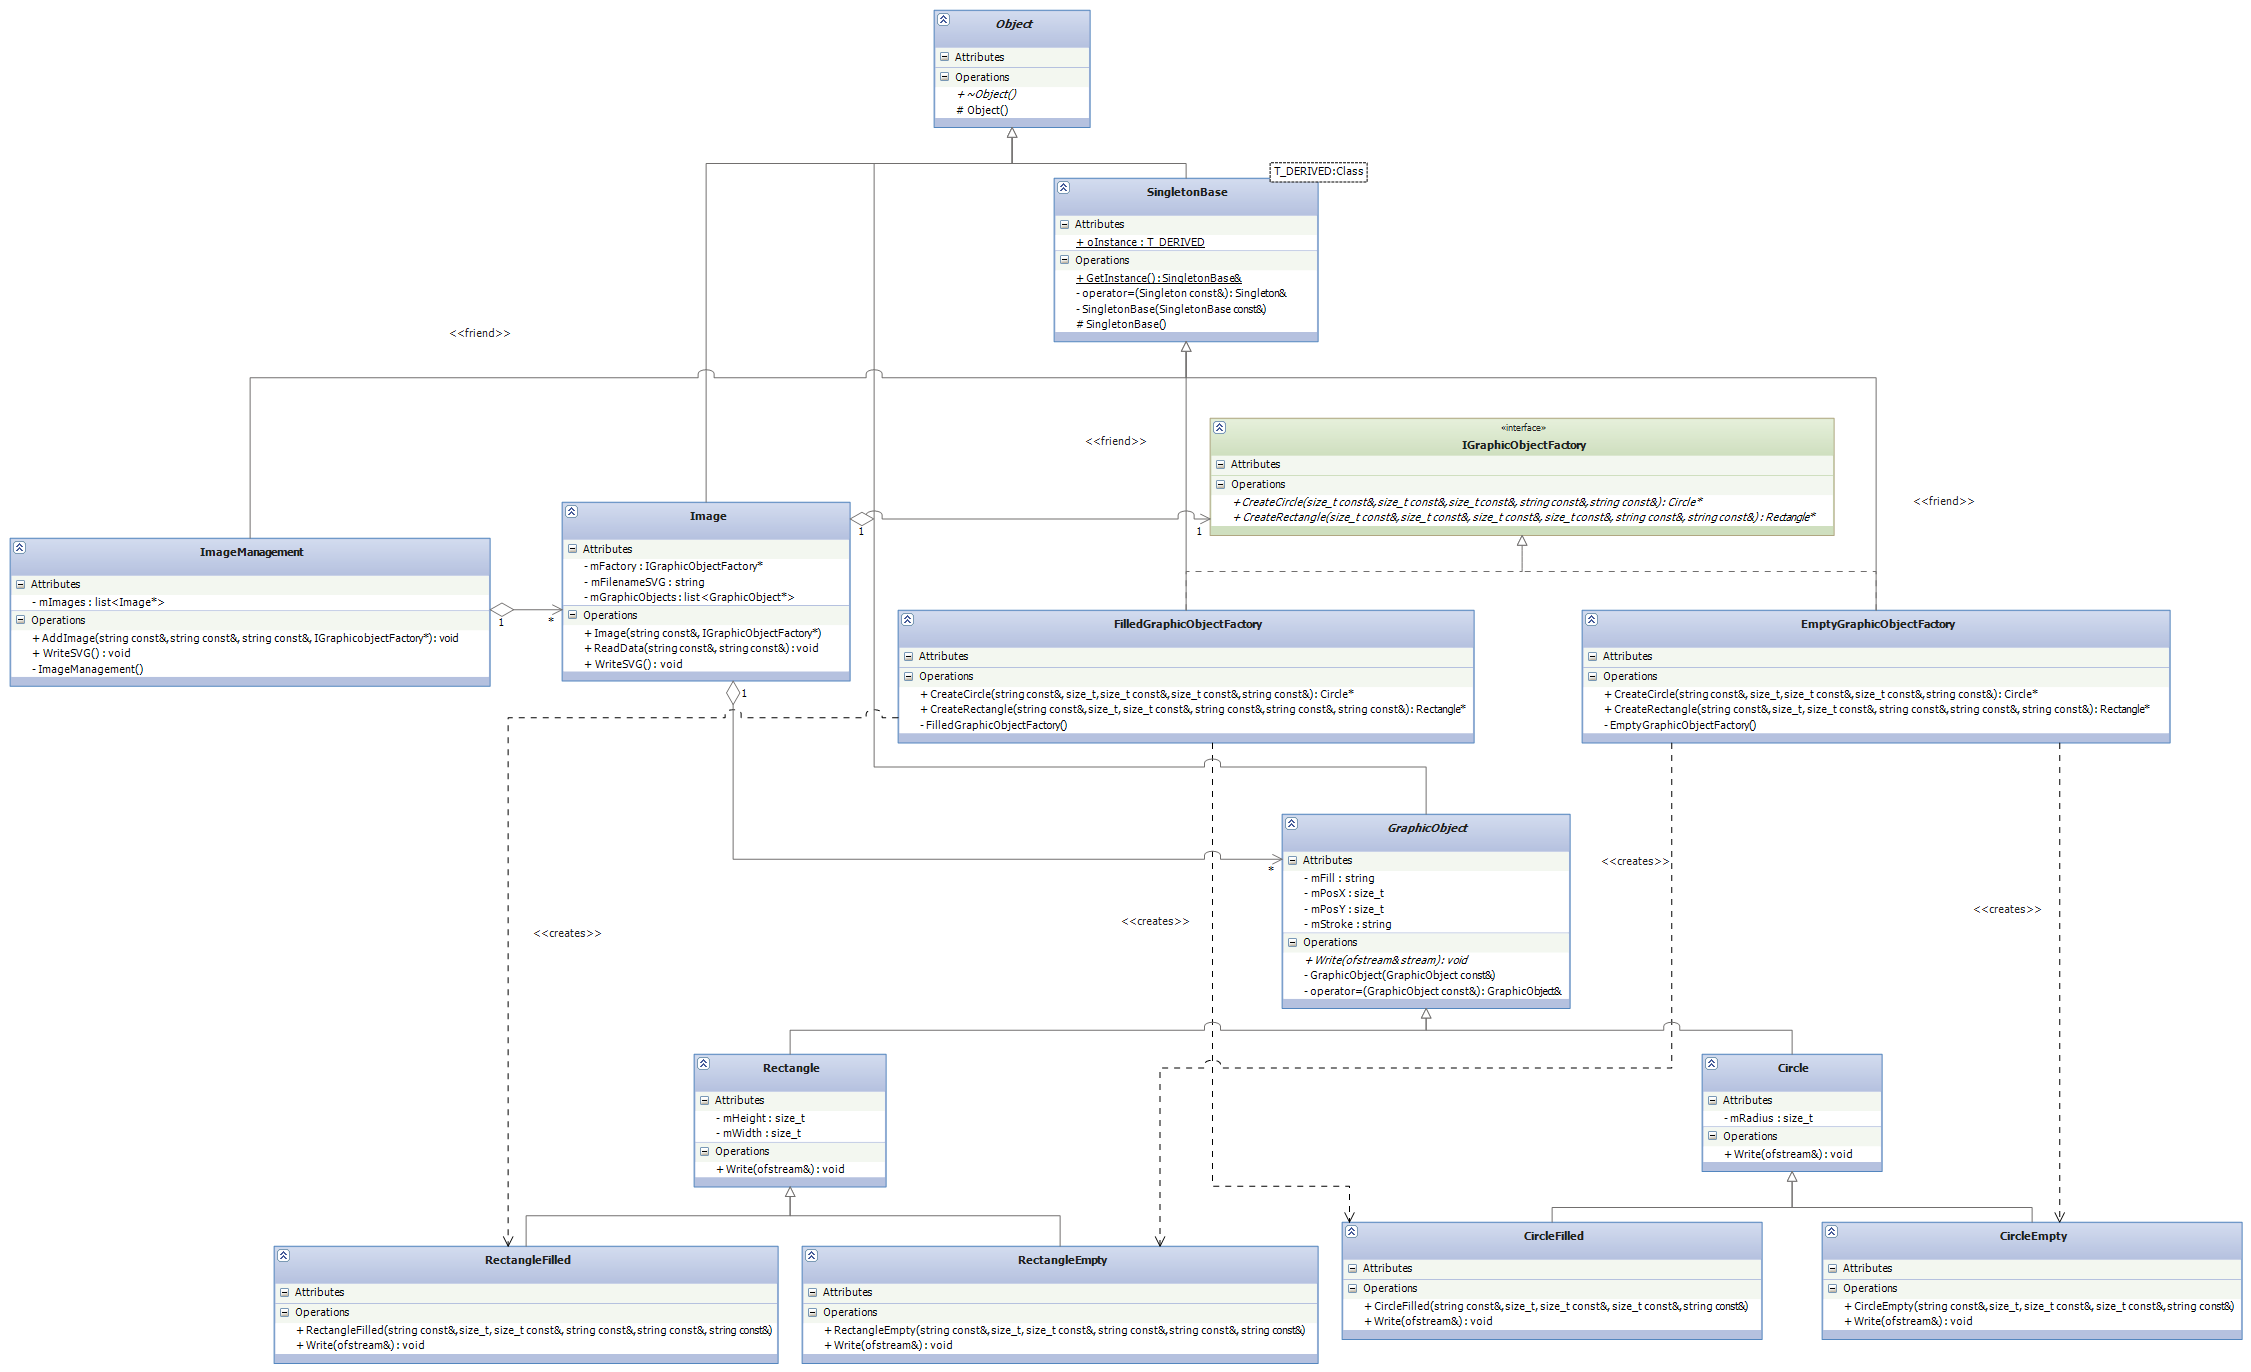
\includegraphics[angle=90,scale=0.4] {../Klassendiagramm.png}

\newpage
\subsection {Komponentenübersicht}
\begin {itemize} 
	\item Klasse "Object":
	\newline
	Basis aller Basisklassen.
	
	\item Klasse "SingletonBase":
	\newline
	Template Basisklasse für Singletons.
	
	\item Klasse "ImageManagement":
	\newline
	Verwaltet die Bilder.
	
	\item Klasse "Image":
	\newline	
	Beinhaltet die einzelnen graphischen Objekte. Kann in eine SVG-Datei geschrieben werden.
	
	\item Interface "IGraphicObjectFactory":
	\newline
	Interface für die Fabrik die die Objekte erzeugt.
	
	\item Klasse "FilledGraphicObjectFactory":
	\newline
	Erzeugt gefüllte graphische Objekte.
	
	\item Klasse "EmptyGraphicObjectFactory":
	\newline
	Erzeugt leere graphische Objekte.
	
	\item Klasse "GraphicObject":
	\newline
	Abstrakte Basisklasse für ein graphisches Objekt.
	
	\item Klasse "Rectangle":
	\newline
	Abgeleitet von GraphicObject. Basisklasse für ein Viereck.

	\item Klassen "RectangleFilled und RectangleEmpty":
	\newline
	Abgeleitet von Rectangle. Vierecke die entweder gefüllt oder leer sind.

	\item Klasse "Circle":
	\newline
	Abgeleitet von GraphicObject. Basisklasse für einen Kreis.

	\item Klassen "CircleFilled und CircleEmpty":
	\newline
	Abgeleitet von Circle. Kreise die entweder gefüllt oder leer sind.
	
	
\end {itemize}

\newpage
\section {Komponentenentwurf}
\subsection {Klasse "Object"}
Abstrakte Basisklasse aller Klassen. Von ihr werden alle anderen Klassen abgeleitet. Beinhaltet einen virtuellen Destruktor.


\subsection {Klasse "SingletonBase"}
Template Basisklasse für die Singletons. Hat einen static Member der auf die Klasse selbst zeigt. Zuweisungsoperator und Copyconstructor sind private. Constructor ist protected.
\\

\textbf {Methode "GetInstance": } 
\newline
Schnittstelle: 
Rückgabetyp: SingletonBase\&.
\newline
Static Function die ein Objekt der Klasse erzeugt und einen Zeiger darauf zurückgibt.
\\

\subsection {Klasse "ImageManagement"}
Hat eine Liste in der die Bilder gespeichert sind. Ist ein Singleton, Constructor ist private.
\\

\textbf {Methode "AddImage": } 
\newline
Schnittstelle: 
Rückgabetyp: void.
\newline
Parameter: string const\& filename1, string const\& filename2, string const\& SVGFileName, IGraphicObjectFactory* factory
\newline
Erzeugt ein neues Bild. Ruft dann die ReadData Funktion des Bildes auf und fügt es zur Liste mit den Bildern hinzu.
\\

\textbf {Methode "WriteSVG": } 
\newline
Schnittstelle:
\newline
Rückgabetyp: void.
\newline
Ruft für jedes Bild WriteSVG auf.
\\

\subsection {Klasse "Image"}
Beinhaltet die Fabrik mit der die Bilder erzeugt werden, den Namen unter der die SVG-Datei gespeichert werden soll und eine Liste mit den graphischen Objekten.
\\

\textbf {Constructor: } 
\newline
Schnittstelle: 
Parameter: std::string const\& str, IGraphicObjectFactory* factory
\newline
Legt die Fabrik und den Dateinamen fest.
\\

\textbf {Methode "ReadData": } 
\newline
Schnittstelle:
\newline
Rückgabetyp: void.
\newline
Parameter: string const\& filename1, string const\& filename2
\newline
Liest die Daten von der Datei mit den Vierecken und der Datei mit den Kreisen ein, erzeugt die Objekte mit der jeweiligen Fabrik und fügt sie dann der Liste mit den Graphischen Objekten hinzu. Wenn fehlerhafte Daten (bei x,y,radius,width,height) in der Datei sind werden diese durch den stringstream in Zahlen umgewandelt. Fill und Stroke werden nicht überprüft. Wenn in der Datei noch zusätzliche Elemente sind, werden diese ignoriert.
\\

\textbf {Methode "WriteSVG": } 
\newline
Schnittstelle: 
\newline
Rückgabetyp: void.
\newline
Öffnet die Datei, schreibt den Header hinein, ruft dann die Write Funktionen von den Graphischen Objekten auf und schreibt zum Schluss den Abschluss in die Datei.
\\


\subsection {Interface "IGraphicObjectFactory"}
Ist die Schnittstelle für die Fabriken, die die gefüllten oder leeren Graphischen Objekte erzeugen.
\\

\textbf {Methode "CreateRectangle": } 
\newline
Schnittstelle: 
\newline
Rückgabetyp: Rectangle*.
\newline
Parameter: size\_t const\& posX, size\_t const\& posY, size\_t const\& width, size\_t const\& height, string const\& stroke, string const\& fill
\newline
Pure virtual function.
\\

\textbf {Methode "CreateCircle": } 
\newline
Schnittstelle: 
\newline
Rückgabetyp: Circle*.
\newline
Parameter: size\_t const\& posX, size\_t const\& posY, size\_t const\& radius, string const\& stroke, string const\& fill
\newline
Pure virtual function.
\\


\subsection {Klassen "FilledGraphicObjectFactory" und "EmptyGraphicObjectFactory"}
Implementieren die Funktionen aus dem Interface. Es wird der Constructor für das entsprechende Graphische Objekt aufgerufen. Je nach dem Kreis/Rechteck gefüllt/leer. Beide sind Singletons.
\\

\subsection {Klasse "GraphicObject"}
Beinhaltet die allgemeinen Information eines graphischen Objekts: Füllung, x-Position, y-Position, Randfarbe. Copyconstructor und Zuweisungsoperator sind private damit das Objekt nicht zugewiesen oder kopiert werden kann.
\\

\subsection {Klasse "Rectangle"}
Hat zusätzlich die Attribute Höhe und Breite des Rechtecks.
\\

\textbf {Methode "Write": } 
\newline
Schnittstelle:
Parameter: ofstream\& stream.
\newline
Rückgabetyp: void.
\newline
Daten werden entsprechend der SVG Syntax in den Stream geschrieben.
\\

\subsection {Klassen "RectangleFilled" und "RectangleEmpty"}
Haben Write Funktionen die noch die entsprechenden Daten zum Stream hinzufügen.
\\

\subsection {Klasse "Circle"}
Hat zusätzlich das Attribut Radius des Kreises.
\\

\textbf {Methode "Write": } 
\newline
Schnittstelle:
Parameter: ofstream\& stream.
\newline
Rückgabetyp: void.
\newline
Daten werden entsprechend der SVG Syntax in den Stream geschrieben.
\\

\subsection {Klassen "CircleFilled" und "CircleEmpty"}
Haben Write Funktionen die noch die entsprechenden Daten zum Stream hinzufügen.
\\

\newpage
\section {Dateibeschreibung}
\subsection {Datei mit Daten für "Rectangle"}
Dateiname: *Rect.data
\newline
Inhalt: Daten für die Vierecke.
\newline
EBNF:
\begin{verbatim}
file = {rectangle}.
rectangle = x y width height stroke [fill].
x = y = width = height = number.
number = digit {digit}.
digit = "0" | "1" | "2" | "3" | "4" | "5" | "6" | "7" | "8" | "9".
stroke = fill = word.
word = letter {letter}.
letter = "a" | "b" | "c" | "d" | "e" | "f" | "g" | "h" | "i" | 
	   "j" | "k" | "l" | "m" | "n" | "o" | "p" | "q" | "r" | 
	   "s" | "t" | "u" | "v" | "w" | "x" | "y" | "z".
\end{verbatim}


\subsection {Datei mit Daten für "Circle"}
Dateiname: *Circ.data
\newline
Inhalt: Daten für die Kreise.
\newline
EBNF:
\begin{verbatim}
file = {circle}.
circle = x y width height stroke [fill].
x = y = radius = number.
number = digit {digit}.
digit = "0" | "1" | "2" | "3" | "4" | "5" | "6" | "7" | "8" | "9".
word = letter {letter}.
letter =  "a" | "b" | "c" | "d" | "e" | "f" | "g" | "h" | "i" | 
	    "j" | "k" | "l" | "m" | "n" | "o" | "p" | "q" | "r" | 
	    "s" | "t" | "u" | "v" | "w" | "x" | "y" | "z".
\end{verbatim}

\newpage
\section {Source Code}

\lstinputlisting[language=C++]{\CodePath Object.h}
\lstinputlisting[language=C++]{\CodePath Object.cpp}
\newpage

\lstinputlisting[language=C++]{\CodePath SingletonBase.h}
\newpage

\lstinputlisting[language=C++]{\CodePath ImageManagment.h}
\newpage
\lstinputlisting[language=C++]{\CodePath  ImageManagment.cpp}
\newpage

\lstinputlisting[language=C++]{\CodePath Image.h}
\newpage
\lstinputlisting[language=C++]{\CodePath Image.cpp}
\newpage

\lstinputlisting[language=C++]{\CodePath IGraphicObjectFactory.h}
\newpage

\lstinputlisting[language=C++]{\CodePath FilledGraphicObjectFactory.h}
\newpage
\lstinputlisting[language=C++]{\CodePath FilledGraphicObjectFactory.cpp}
\newpage

\lstinputlisting[language=C++]{\CodePath EmptyGraphicObjectFactory.h}
\newpage
\lstinputlisting[language=C++]{\CodePath EmptyGraphicObjectFactory.cpp}
\newpage

\lstinputlisting[language=C++]{\CodePath GraphicObject.h}
\newpage
\lstinputlisting[language=C++]{\CodePath GraphicObject.cpp}
\newpage

\lstinputlisting[language=C++]{\CodePath Rectangle.h}
\newpage
\lstinputlisting[language=C++]{\CodePath Rectangle.cpp}
\newpage

\lstinputlisting[language=C++]{\CodePath RectangleFilled.h}
\newpage
\lstinputlisting[language=C++]{\CodePath RectangleFilled.cpp}
\newpage

\lstinputlisting[language=C++]{\CodePath RectangleEmpty.h}
\newpage
\lstinputlisting[language=C++]{\CodePath RectangleEmpty.cpp}
\newpage

\lstinputlisting[language=C++]{\CodePath Circle.h}
\newpage
\lstinputlisting[language=C++]{\CodePath Circle.cpp}
\newpage

\lstinputlisting[language=C++]{\CodePath CircleFilled.h}
\newpage
\lstinputlisting[language=C++]{\CodePath CircleFilled.cpp}
\newpage

\lstinputlisting[language=C++]{\CodePath CircleEmpty.h}
\newpage
\lstinputlisting[language=C++]{\CodePath CircleEmpty.cpp}
\newpage

\lstinputlisting[language=C++]{\CodePath main.cpp}
\newpage


\section {Testausgaben} 

\begin {verbatim}
Testcase0: Not existing files
AddImage(Filled) ... Image.cpp::ReadData: 
File with Rectangle Data couldn't be opened
done
AddImage(Empty) ... Image.cpp::ReadData: 
File with Rectangle Data couldn't be opened
done
WriteSVG ... done

Testcase1: Empty files
AddImage(Filled) ... done
AddImage(Empty) ... done
WriteSVG ... done

Testcase2: Files with correct data
AddImage(Filled) ... done
AddImage(Empty) ... done
WriteSVG ... done

Testcase3: Files with wrong data
AddImage(Filled) ... done
AddImage(Empty) ... done
WriteSVG ... done
\end {verbatim}


\end{document}